\chapter{Specifying and Synthesizing a New Term Rewriting System}
\label{chapter:synthfromscratch}

In the simplifier work, we devised a reduction order to prove that the simplifier ruleset was guaranteed to terminate, and then made use of that order in synthesizing new rules for that ruleset. In a way, we could consider this an extended instance of programming by demonstration---we received around a thousand example programs, manually derived a specification that described all of those examples, and then used it to synthesize new programs. The natural question to ask is whether a user might simply write the specification and synthesize their desired TRS without seeding it with any handwritten rules at all.

In this chapter, we argue that the reduction order is a useful and powerful way of writing specifications for term rewriting systems. We demonstrate this using the Halide variable solver term rewriting system as a case study. First we will discuss the rationale behind using reduction orders as specifications and the design of our synthesis pipeline. We define some possible reduction orders that represent strategies or gradients along which to rewrite expressions to bring them closer to the desired solved form with regard to the specified variable. We then evaluate these orders by synthesizing entirely new term rewriting systems using the orders as specifications and evaluating their performance on a suite of benchmarks.

\begin{figure}
\begin{tikzpicture}[<->,auto,node distance=6cm]
\tikzstyle{every state}=[draw=none]
\node[state]    (A)     {$(y + x) - y$};
\node[state]    (B) [below left of=A]    {$x + 0$};
\node[state]    (C) [below right of=A]    {$x + (y \cdot (z - z))$};
\node[state]    (D) [right of=A]    {$x \cdot (\frac{z}{z})$};
\node[state]    (E) [above of=D]    {$x$};
\node[state]    (F) [above left of=A]    {$\hmin(x, x \cdot 1)$};
\node[state]    (G) [left of=A]    {$\frac{x \cdot 3}{3}$};

\path (A)   edge    node {} (B)
            edge    node {} (C)
            edge    node {} (D)
            edge    node {} (E)
            edge    node {} (F)
            edge    node {} (G)
     (B)    edge [bend right]   node {} (C)
            edge [bend right]   node {} (D)
            edge [bend right]   node {} (E)
            edge    node {} (F)
            edge    node {} (G)
    (C)     edge    node {} (D)
            edge    node {} (E)
            edge [bend right]   node {} (F)
            edge    node {} (G)
    (D)     edge [bend right]   node {} (E)
            edge [bend right]   node {} (F)
            edge [bend right]   node {} (G)
    (E)     edge [bend right]   node {} (F)
            edge [bend right]   node {} (G)
    (F)     edge [bend right]   node {} (G);

\end{tikzpicture}
\end{figure}


\subsection{Rationale for synthesis pipeline}

Here we lay out the rationale for our proposed synthesis pipeline. In particular, we will discuss three key assumptions: that a reduction order can be an effective heuristic for guiding term rewrites to a desired form; that a term rewriting system can be synthesized incrementally rule by rule; and that choosing candidate left-hand sides gathered from realistic inputs is an efficient means of finding rules that will have high impact on the performance of the term rewriting system.

When we specify a term rewriting system in this work, we say that it must have three properties:

\begin{itemize}
    \item it must be semantics-preserving
    \item it must terminate on all inputs
    \item it must rewrite terms into a form that has some desired property
\end{itemize}

The first two properties are required. As our language is undecidable, we can't create a TRS that is able to rewrite \emph{all} terms into the desired form. Our incremental synthesis pipeline is thus designed to grow the ruleset rule by rule, such that with each successful iteration of the synthesis algorithm, the ruleset is able to move more terms further toward the desired form.

In chapter~\ref{chapter:synthesis}, we showed that the Halide simplifier was semantics-preserving by verifying that for each rule $(l \rewrites r) \in R$, $l =_e r$, where the equality relation $=_e$ was checked via an SMT solver. We showed that the TRS was terminating by choosing an order $>$ over terms and showing that every rule in $R$ rewrote terms to be strictly less in that order. When we synthesized new rules to add to the simplifier ruleset, we did not explicitly define the third criterion, but allowed the termination order fitted to the existing ruleset to guide the synthesis pipeline. 

In this section, we will define more precisely the goal or intent behind a term rewriting system. We argue that an effective means of specifying this intent for the purpose of synthesis is to use a reduction order to capture the notion of rewriting a term to be closer to some goal state.

\begin{figure}
    \centering
\subfigure[$\termlang$]{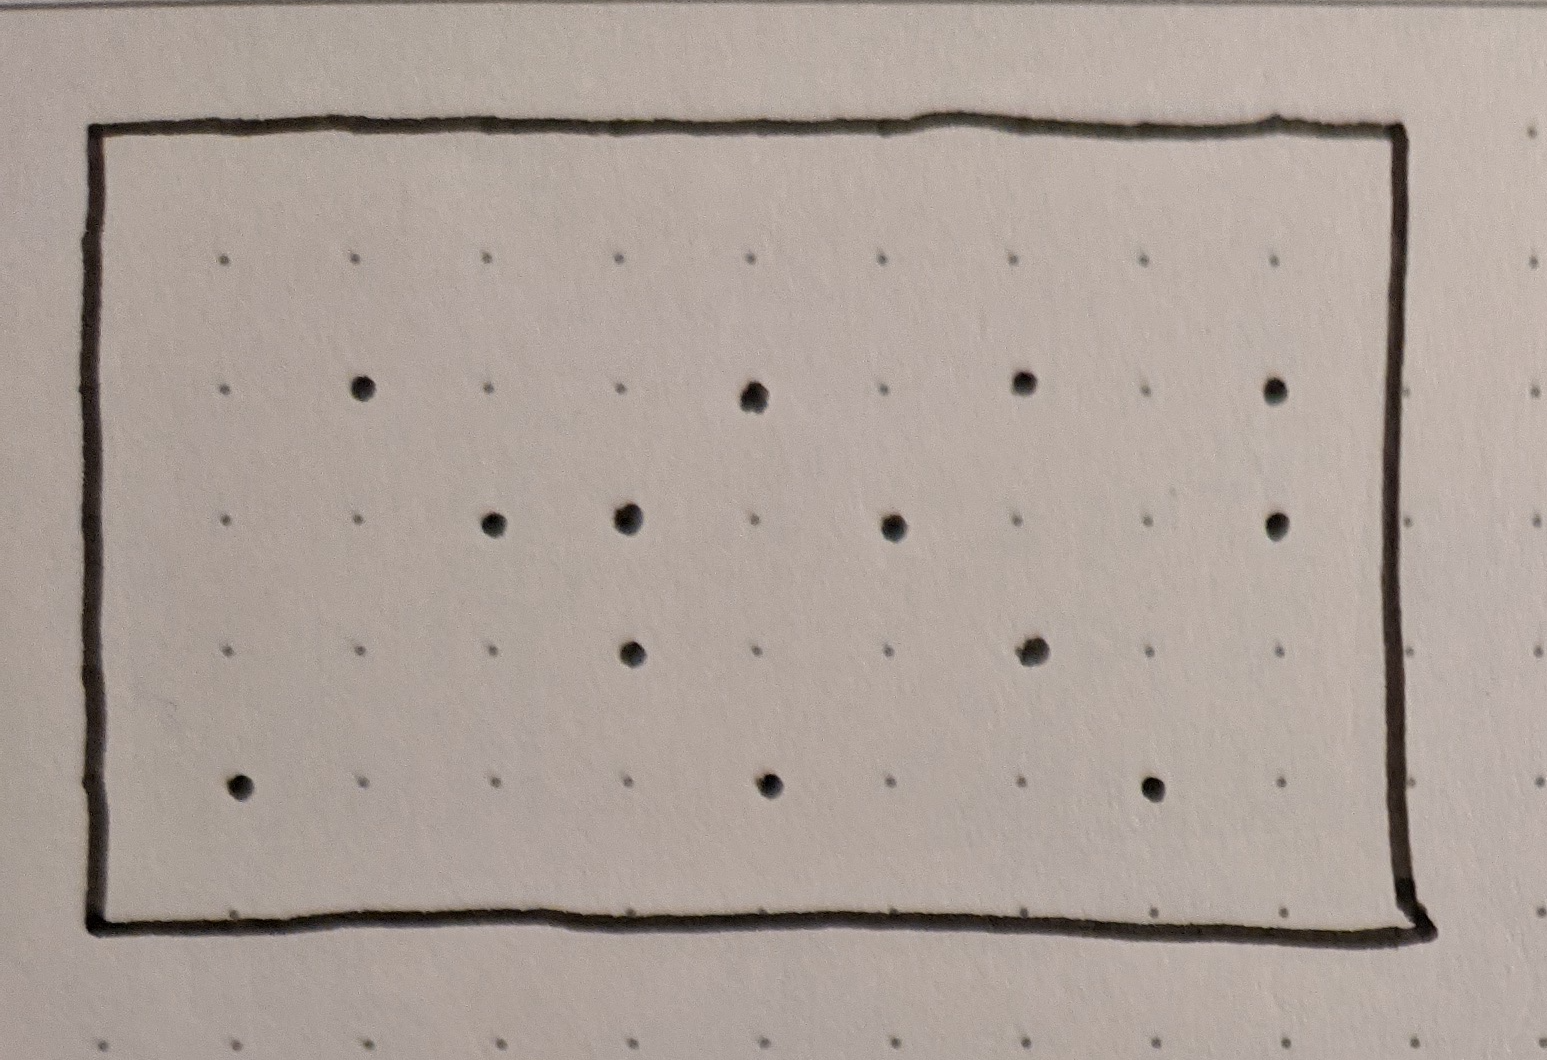
\includegraphics[width=0.3\textwidth]{figures/diagram1.png}}
    \hspace{1em}
    \subfigure[$\{s | s \in \termlang \wedge \phi(s)\}$ in red]{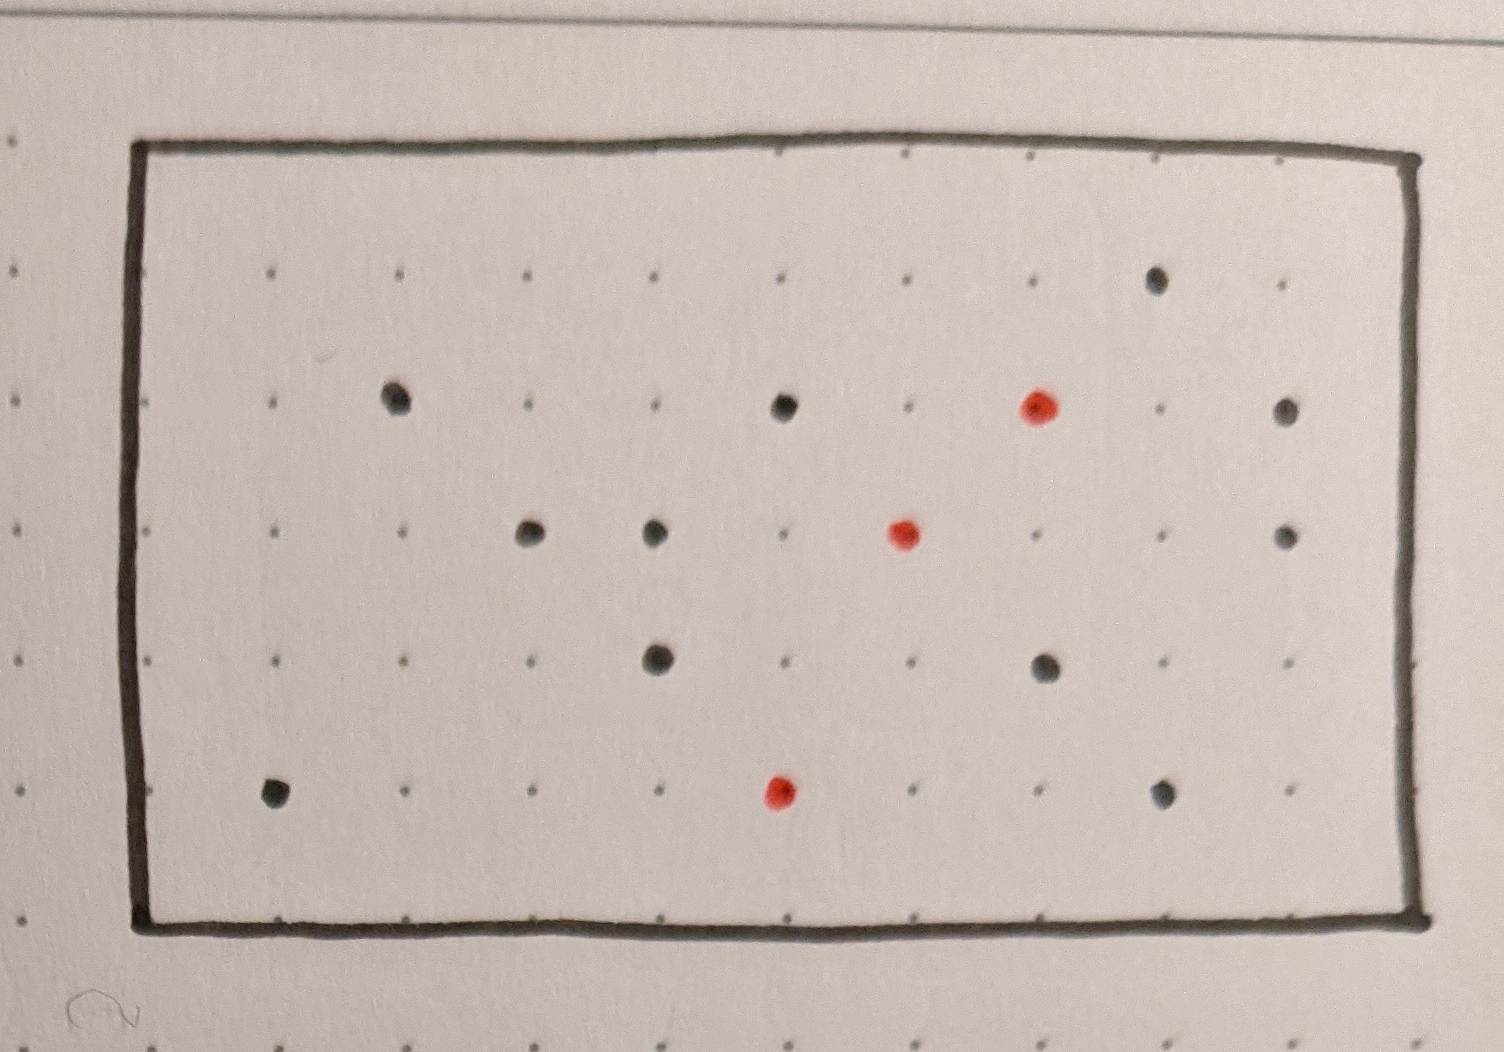
\includegraphics[width=0.3\textwidth]{figures/diagram2.png}}
    \hspace{1em}
    \subfigure[$\goallang$ in blue]{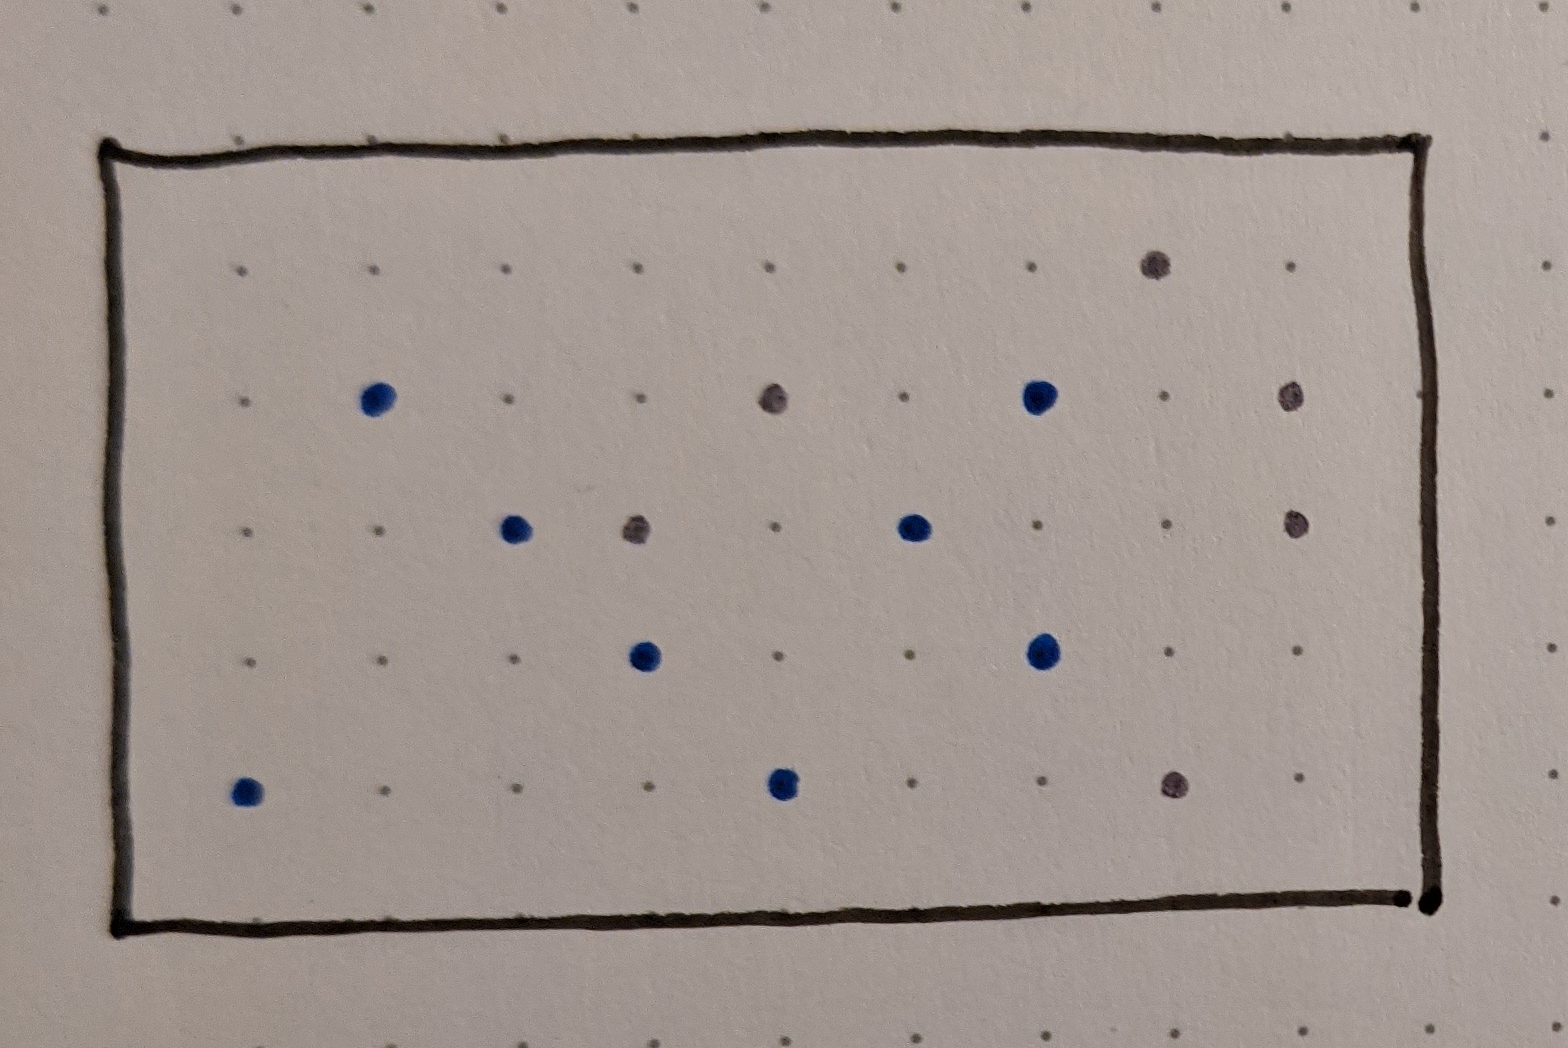
\includegraphics[width=0.3\textwidth]{figures/diagram3.png}} \\
    \subfigure[Undirected edges connect all $s, t$ st. $s =_e t$]{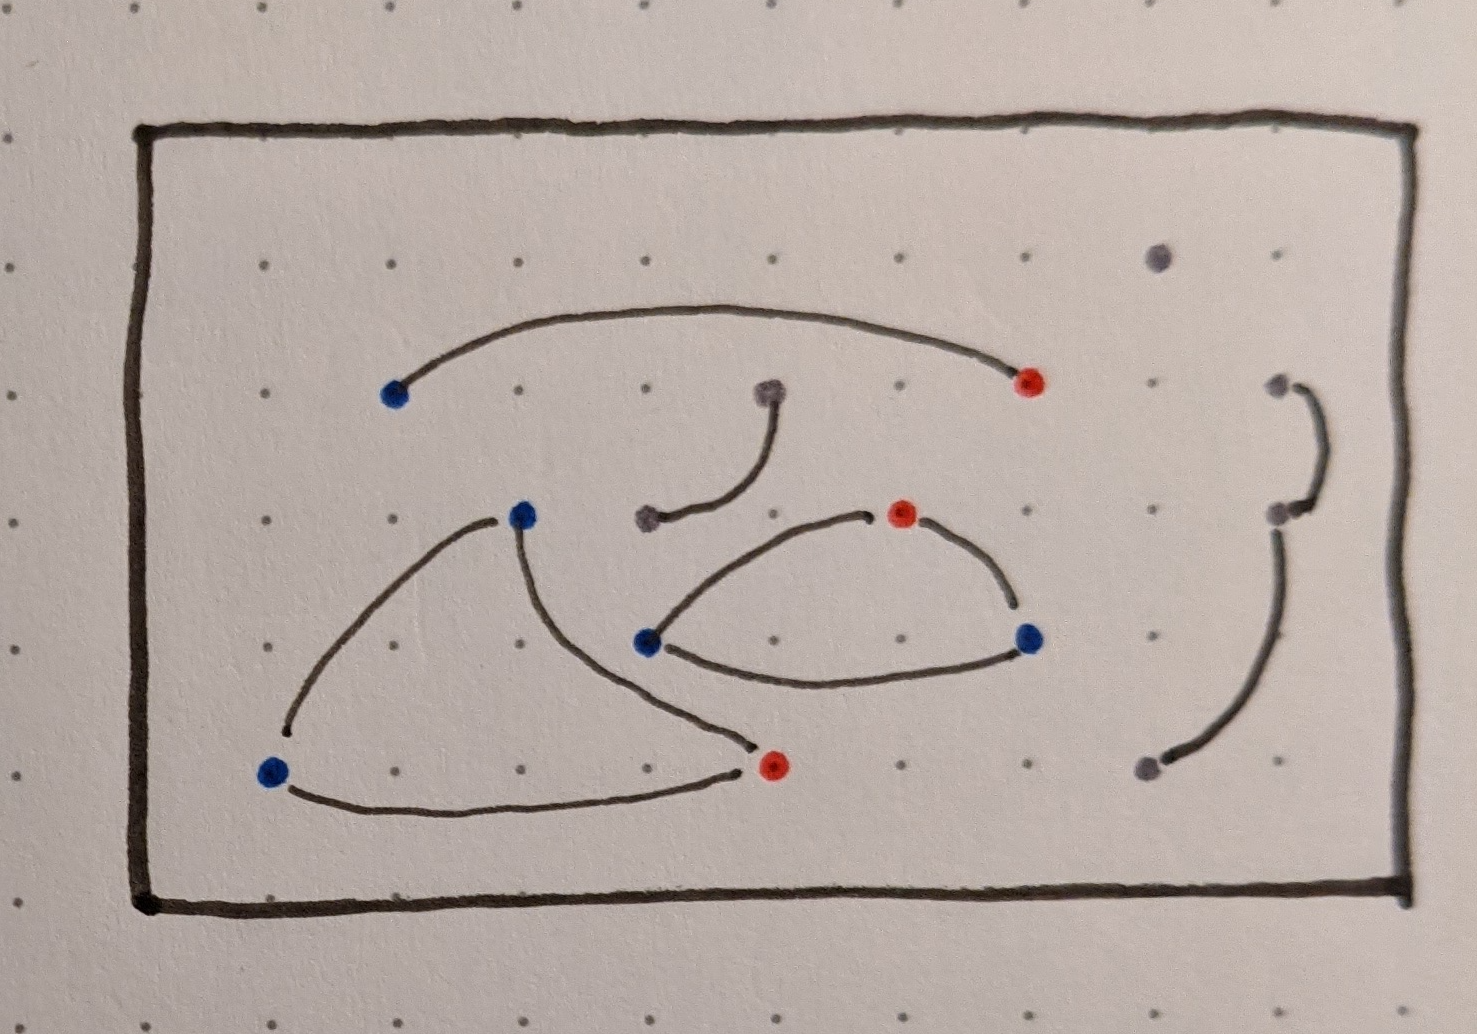
\includegraphics[width=0.3\textwidth]{figures/diagram4.png}}
    \hspace{1em}
    \subfigure[Directed edges connect all $s, t$ st. $s =_e t \wedge s > t$]{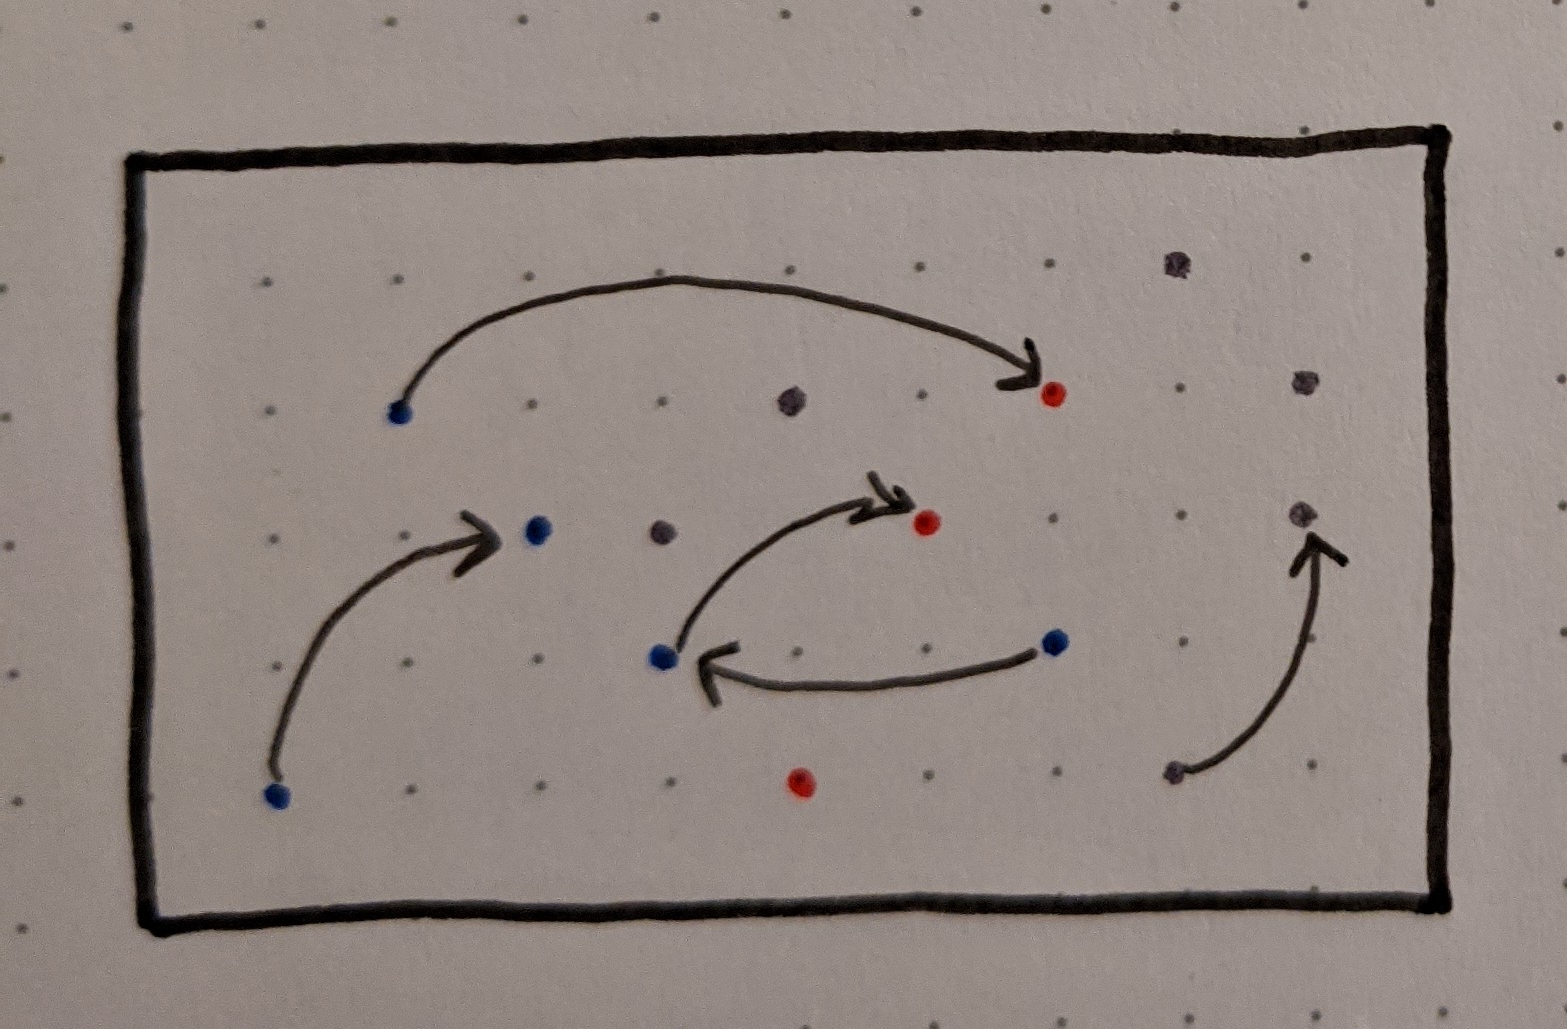
\includegraphics[width=0.3\textwidth]{figures/diagram5.png}}
    \caption{Each dot in (a) represents a term in $\termlang$. In (b), each term in the goal state is drawn in red. In (c), all terms which are equivalent to a term in the goal state ($\goallang$) are drawn in blue. The goal of the term rewriting system is to rewrite all blue dots in (c) to a red dot in (b). In (d), undirected edges connect all pairs of terms that are semantically equivalent. In (e), those edges have been oriented with a reduction order. Given the specification $\forall (l \rewrites r) \in R \st l =_e \wedge l > r$, we can find a TRS $R$ by picking a finite subset of all the directed edges in (e).}
    \label{fig:termuniverse}
\end{figure}

First, we define the goal property that describes the underlying intention of the term rewriting system. Assume some language of terms $\termlang$ and a semantic equivalence relation over those terms $=_e$ (as opposed to a syntactic equivalence relation, which we will write $=$). We write the goal property as a predicate function $\phi$ such that $\phi(s)$ is true if $s$ is in the goal state and false otherwise. 

We can thus write the domain of the term rewriting system as a language $\goallang \subseteq \termlang$, defined as

\[
\goallang = \{s | s \in \termlang \wedge (\exists t \in \termlang\;.\; s =_e t \wedge \phi(t))\}
\]

We want our term rewriting system to put every term in $\goallang$ into a form that satisfies our goal function $\phi$. When we specify how a term rewriting system rewrites terms into a goal state, we refer only to terms in $\goallang$; when the TRS rewrites a term that in is $\termlang$ but not in $\goallang$, it need only obey the semantics-preserving and termination properties.\footnote{We might prefer that the term rewriting system act on terms not in $\goallang$ as little as possible, but this is purely for performance reasons and can be set aside for now.}

To illustrate these definitions, we will develop formal specifications for two example term rewriting systems that represent different aspects of the Halide simplifier TRS. As discussed in section~\ref{sec:uses-of-trs}, the simplifier is used in many places in the Halide compiler under a number of difference circumstances, perhaps explaining the extremely complex reduction order we devised to fit its ruleset. Here, we will isolate two of the simplifier's important function: showing that a term must always evaluate to true, and showing that a term is strictly increasing or strictly decreasing.

 As in the rest of this work, we assume that $\termlang$ is the Halide expression grammar. First, we consider a prover TRS, which tries to determine if an expression is equivalent to the booleans values true or false, or if its truth value is unknown. We state that the prover has a domain language $\goallang_P$, which contains all terms in the Halide expression language that are equivalent ($=_e$) to $\htrue$ or $\hfalse$, and a goal state function $\phi_P$ that returns true if its input syntactically equivalent ($=$) to $\htrue$ or $\hfalse$ and false otherwise. This goal function encodes the purpose of the TRS, which is to transform all terms that are semantically equivalent to true or false to the boolean constants $\htrue$ or $\hfalse$. (Again, the goal function says nothing about terms in the Halide language, e.g. $x < y$, that are not provably true or provably false.)

\begin{align*}
    \phi_P(s) := s = \htrue \vee s = \hfalse
    \goallang_P = \{s | s \in \termlang \wedge (s =_e \htrue \vee s =_e \hfalse)\} \\
\end{align*}

The second example is a TRS that seeks to show that a given expression is monotonic. The goal function for this TRS is a bit more subtle. The Halide compiler's means of querying the monotonicity of an expression is sound but not complete: it walks the expression to see if it is in a syntactic form that can be recognized as monotonically increasing, monotonically decreasing, or constant. If it cannot recognize the expression as any of these three, it returns unknown. The job of the monotonic rewriter TRS is to put expressions into this syntactic form wherever possible. We say then that the domain language of the monotonic rewriter $\goallang_M$ is all terms $s$ in $\termlang$ where there exists some term $t$ such that $s =_e t$ and $t$ is in a syntactic form that can be recognized as monotonic or constant by the function $\texttt{is_monotonic}$ in the Halide codebase. The goal state function $\phi_M$ returns false when $\texttt{is_monotonic}$ returns unknown on an input term, and true otherwise. (Again, $\phi_M$ may return false for a term that is not in monotonic form because it is not in $\goallang_M$, i.e. no semantically equivalent monotonic form exists, but we can disregard this case for now.)

With these definitions in hand, we are now ready to formally specify the three properties we require of a term rewriting system (semantics-preserving, terminating, and rewrites terms into a desired form). We write $R(s)$ for the output of a term rewriting system $R$ on the input term $s$. Assume we use the means of assuring semantics preservation and termination as used above. Then, for an equivalence relation $=_e$ and a goal function $\phi$, we write that a specification for an ideal TRS $R$ thus:

\begin{align*}
\forall s \in \goallang \st \phi(R(s)) \wedge \\
\forall t \in \termlang \st t =_e R(t) \wedge R(t) \textrm{ terminates }
\end{align*}

Of course, since our theory is undecidable, the $\forall s \in \goallang \st \phi(R(s))$ portion of our specification is almost certainly unrealizable in the general case. Instead, we would like to encode a means of making progress towards this goal, rather than ruling out all TRSs that do not achieve it. We can think of this as a strategy for rewriting terms to be closer to the desired goal state. For example, imagine we started writing rules for the prover, and started with this pair:

\begin{align*}
    x = x \rewrites \htrue \\
    x + (y - y) \rewrites x
\end{align*}

We might note that the second rule is canceling like terms, and add many more rules that do the same. If we wanted to formally encode this strategy, we could do so using an order over terms, such that terms that satisfy the goal condition $\phi$ would be least elements in that order. In the case of the prover, the order could be to compare terms by their length; since the boolean constant $\htrue$ is of the shortest possible length in the Halide expression language, it is a least element of this order. Let us call such an order $\goalorder$ and add it as a condition to our specification:

\begin{align*}
\forall s \in \goallang \st \phi(R(s)) \wedge  s \geq_{\phi} R(s) \wedge \\
\forall t \in \termlang \st t =_e R(t) \wedge  R(t) \textrm{ terminates }
\end{align*}

As pictured in figure~\ref{fig:termuniverse}, the process of choosing rewrite rules for a ruleset is choosing edges from the graph (d) and orienting them. The goal order $\goalorder$ could be considered an order traversal from terms not in the goal state to terms that are. 

Now, assume we have been given some solution to our specification in the form of a term rewriting system $R$. How can we prove that it fulfills our criteria? In prior work, we proved that a term rewriting system was semantics-preserving ($\forall t \in \termlang \st t =_e R(t)$) and terminating ($\forall t \in \termlang \st R(t) \textrm{ terminates }$) by showing that those properties held over every rule in the ruleset. We can use a similar strategy here: if the goal order $\goalorder$ holds for every rule in $R$, then it must hold for all of $R$ as a whole.

\begin{assumption}
We can lower our requirement that the ruleset $R$ rewrite every term in $\goallang$ to the goal state to the requirement that every rule in $R$ rewrites terms to be closer to the goal state, as described by a goal order $\goalorder$.
\end{assumption}

% describe this more clearly: 
Requiring the goal order hold over every rule in $R$ will exclude some possible term rewriting systems for which the goal order would hold over the full system, just as requiring that the termination property hold over every rule in $R$ excludes some TRSs that are terminating. This is illustrated in figure~\ref{fig:termuniverse}; when we choose an order that turns the undirected edges in (d) to directed edges in (e), there are now some terms in $\goallang$ that are unable to reach a goal state. However, checking that this property holds over every rule can be done quickly and automatically. Just as with the termination guarantee, so long as every rule we add to a ruleset conforms to the goal order, we can add, delete, or permute the priority of rules without fear of losing our overall guarantee. This quick machine-checkable proof allows us to synthesize a TRS without human supervision.

In order for the goal order to hold over every term that may match and be rewritten by a rule, it must be a valid reduction order: well-founded, $\Sigma$-operation compatible, and closed under substitution (see~\citep{baader1999term}). Usefully, this means we do not need a separate termination order; since a goal order requires that each rewrite moves a term monotonically lower in the order, it also provides a termination guarantee.

We can now restate our term rewriting system specification like so:

\begin{align*}
    \forall s \in \goallang \st \phi(R(s)) \wedge \\
    \forall (l \rewrites r) \in R \st l =_e r \wedge l \goalorder r
\end{align*}

Since any term rewriting system we wish to synthesize will be semantics-preserving, the major decision we need to make in specifying a term rewriting system is to pick a goal order:

\begin{assumption}
We can effectively formalize the goal of a term rewriting system by choosing a \emph{goal order} over terms such that, for two terms $s$ and $t$ such that $s \goalorder t$ in this order, $t$ is assumed to be closer to the goal state.
\end{assumption}

Finding a goal order that encodes progress towards a goal state is a difficult task, and requires human intuition and ingenuity. Our work does not directly aid in this task, which is still up to the human author of the term rewriting system; however, our synthesizer machinery can aid in experimenting with and selecting goal orders.

\begin{table}[]
    \centering
    \begin{tabular}{|l|l|l|}
    \hline 
        TRS & Goal function $\phi$ & Goal order $>$ \\
        \hline 
        Prover &  $\phi(s)$ if $s$ is $\htrue$ or $\hfalse$ & $s > t$ if $t$ is shorter than $s$\\
        \hline
        Monotonic rewriter & $\phi(s) := \texttt{is_monotonic(s)}$ & $s > t$ if $s$ has more $\%$ ops \\
                 & & $s > t$ if $s$ has more constants \\
        \hline
    \end{tabular}
    \caption{Two term rewriting systems, goal functions that encode their intent, and goal orders that represent moving towards those goals}
    \label{tab:trsspecs}
\end{table}

As discussed above, the prover could adopt a strategy of making expressions shorter, with the aim of eventually being able to reduce them to the constants $\htrue$ or $\hfalse$. For the monotonic rewriter, one expression in the goal state is $x \cdot c_0$ where $c_0$ is a positive constant; the monotonicity checker recognizes this form as monotonically increasing. So, one possible strategy could be to move constants to the right side of an equation wherever possible. We may also want to employ sub-strategies: if the prover TRS contains the rule $x = x \rewrites \htrue$, we might choose a strategy of putting expressions into a kind of canonical form wherever possible, so we can rewrite an expression $e_1 = e_2$ into $e' = e'$ and then apply the identity rewrite rule. The simplifier reduction order, which was composed of several orders lexicographically, could be said to employ a series of sub-strategies in this way. See table~\ref{tab:trsspecs} for the prover and monotonic rewriter goal functions and some goal orders that approximate them.
 % check with Andrew about monotonic rewriter example

If we accept the assumption that a reduction order can encode the strategy of rewriting a term to be closer to our goal, we now have a specification that should hold for every individual rule we synthesize:

\[ \forall (l \rewrites r) \in R \st l =_e r \wedge l \goalorder r
\]

The set of possible rules made up of terms in the Halide expression language that conform to that spec is still infinitely large. The other part of our spec required that $\forall s \in \goallang \st \phi(R(s))$, but this is unrealizable. Instead we relax to a specification that could actually be checked; for example, we could fix a set $S$ of terms and write that our term rewriting system should:

\begin{align*}
    \forall s \in S \st \phi(R(s)) \wedge \\
    \forall (l \rewrites r) \in R \st l =_e r \wedge l \goalorder r
\end{align*}

Now we have a realizable synthesis procedure: we can synthesize rules $(l \rewrites r)$ such that $l =_e r \wedge l \goalorder r$, add them to $R$, and terminate when $\forall s \in S \st \phi(R(s))$ holds, as described in algorithm~\ref{algo:synthesis}. In practical cases, we may want to use other termination conditions, such as requiring that some fraction of $S$ can be solved. In our prior work, we did not check that the outputs of the synthesis-augmented simplifier brought previously unsolved terms to the goal state at all, but relied on a fairly complex goal order to produce a strengthened ruleset that was demonstrably more effective on our benchmarks.

Finally, we need a strategy for choosing which rule to add to growing ruleset at each step. As the space of potential rules is so large, even if term sizes are bounded, simply sampling at random may not be effective. Our synthesis pipeline defines a strategy for growing a ruleset so that it is able to rewrite more and more of $\goallang$, in a way that is of practical benefit to the compiler. In prior work, we gathered a corpus of expressions seen by the compiler in realistic circumstances and mined them for general patterns to form candidate LHS terms. We then attempted to synthesize RHSs for each candidate LHS term to form rules. We assert that this is an effective method of creating a ruleset is effective under realistic workloads.

\begin{assumption}
An effective heuristic for choosing candidate left-hand side terms for new rules is to gather expressions seen by the compiler under realistic circumstances and mine them for general patterns.
\end{assumption}

Note that when we gathered input expressions in prior work, we did not check to see if those expressions were in the TRS domain $\goallang$. Any means of checking membership in $\goallang$ is necessarily incomplete, so any ruleset learned from a checked input list would inherit the incompleteness of the checker. Also, note that we will want to rewrite subterms of expressions that are not themselves in $\goallang$: in the prover TRS, although all input expressions are boolean-valued, we will want to rewrite subterms of all possible types. For example, given the ruleset $R = \{x = x \rewrites \htrue, x + x \rewrites x \cdot 2\}$, we need the second rule that rewrites a numeric-valued expression so that we can rewrite $x + x = x \cdot 2$ to $\htrue$.

Given these three assumptions, we propose the synthesis pipeline in algorithm~\ref{algo:synthesis}. 

\subsection{The Halide variable solver}

The Halide simplifier was a fairly mature system, in production for over a year and consists of almost a thousand rules. The Halide variable solver, by contrast, is a much smaller system, currently implemented as a series of if statements rather than a formal term rewriting system, and consisting of the equivalent of less than a hundred rules. The simplifier's use cases were quite varied and complex, and the existing ruleset required a complex composite reduction order to cover their full purpose. The variable solver is much smaller and more focused and can be captured by much simpler reduction orders. With the variable solver, therefore, we have the opportunity to experiment with various reduction orders to find the one that fulfills the system's purpose best, and to synthesize a TRS entirely from scratch, rather than augment an existing system.

% synthesis pipeline: Rosette, encoding reduction order as metasketches, metasketch search order, etc
% discussion of different granularities of reduction order
% evaluation of various synth'd TRSs

\section{The variable solver reduction orders}

Here we refer to \emph{target-matching variables} as variables that can be unified with the target variable or subterms that contain the target variable. Variables that cannot be unified with the target variable or subterms that contain the target variable are called \emph{non-target-matching variables}. All variables that occur in the variable solver ruleset are either target-matching or non-target-matching. Allowing variables that can match either target variable-containing subterms or non-target variable containing subterms complicates reduction order definitions. \jln{is it true that any rule containing variables that can match anything can be replaced by multiple rules that only contain target-matching or non-target-matching variables?}

We represent target-matching variables as $x^t, y^t$, etc., and non-target-matching variables as $x^n, y^n$, and so on.

\subsection{Reduce occurrences of target-matching variables}

\[ s_1 >_t s_2 \iff \forall x^t \in \mathcal{V}(s_1) |s_1|_{x^t} \geq |s_2|_{x^t}
\]

The proof that this order is a valid reduction order is straightforward. The order is clearly well-formed, since $|s|_{t_i}$ has a minimum value of 0. The order is compatible with $\Sigma$-operations; for any

\[ s_1 >_t s_2 \implies f(t_1,...t_{i-1},s_1,t_{i+1},...,t_n) >_t f(t_1,...t_{i-1},s_2,t_{i+1},...,t_n)
\]

\begin{align*}
\sum_{x^t \in \mathcal{V}} \sum_{0}^{i - 1} |t_k|_{x^t_k} + |s_1|_{x^t_k} + \sum_{i + 1}^{n} |t_k|_{x^t_k} >
\sum_{x^t \in \mathcal{V}} \sum_{0}^{i - 1} |t_k|_{x^t_k} + |s_2|_{x^t_k} + \sum_{i + 1}^{n} |t_k|_{x^t_k}
\end{align*}

Since $|s|_{x^t}$ is always non-negative, the implication clearly holds.

Finally, the order is closed under substitutions. A substitution $\sigma$ could increase the number of target-matching variables in $s_2$ by replacing some $x^t$ with a subterm containing multiple target-matching variables, but since all target-matching variables in $s_2$ must occur an equal or greater number of times in $s_1$, the order must be preserved. Any substitution for a non-target-matching variable will have no effect on the number of target-matching variables in $s_1$ or $s_2$ by definition. 

Note that this order does not require that the number of non-target-matching variable occurrences in $s_1$ be equal or greater to the number of occurrences in $s_2$; it is perfectly fine to increase the size of the rewritten expression so long as the count of target-matching variables goes down. For example, the rule $t_0 <= (t_0 + n_1) \rewrites n_1 >= 0$ introduces a new constant on its RHS, but obeys the order as it reduces the number of occurrences of $t_0$.

\subsection{Move occurrences of target-matching variables to the left}

The intuition behind the order is simple, but we will have to take care in our definition to make sure it is a valid reduction order. We define this order by transforming terms into strings and then comparing the strings lexicographically.

To transform a term into a string (we write this function as $\texttt{varstr}(s)$), we first take the sequence of all occurrences of variables and constants in the term, in the order in which they occur. We truncate the sequence by removing everything after the last occurrence of a target-matching variable. We then replace all target-matching variables with 'a' and all non-target-matching variables or constants with 'b', and compare the resulting string with that of another term in lexicographic order (such that a $<$ b).

\begin{tabular}{l|l|l|l}
\centering
$n_0 + t_0 > t_0 + n_0$ & $(n_0 t_0) > (t_0 n_0)$ & $(n_0 t_0) > (t_0)$ & ab $>$ a \\
\end{tabular}

This order is clearly compatible with $\Sigma$-operations; if $\texttt{varstr}(s_1) > \texttt{varstr}(s_2)$, then the order will still hold if identical prefixes and suffixes are added to both terms. 

\begin{align*}
s_1 > s_2 \implies & f(t_1,s_1,t_n) > f(t_1,s_2,t_n) \\
\texttt{varstr}(s_1) > \texttt{varstr}(s_2) \implies & \texttt{varstr}(t_1) + \texttt{varstr}(s_1) + \texttt{varstr}(t_n) > \\
&\texttt{varstr}(t_1) + \texttt{varstr}(s_2) + \texttt{varstr}(t_n)
\end{align*}

However, we need to add an additional condition to make the order closed under substitution. Consider a rule

\[ (n_0 + n_1) + (t_0 + n_2) \rewrites (n_2 + t_0) + (n_0 + n_1)
\]

The rule appears to move the target-matching variable to the left and thus seems to be in conformance with the order. However, given the substitution $\sigma = \{ n_0 \mapsto y^n, n_1 \mapsto z^n, t_0 \mapsto x^t, n_2 \mapsto ((u^n + v^n) + w^n)\}$, we obtain the transformation
\[ (y^n + z^n) + (x^t + ((u^n + v^n) + w^n)) \rewrites (((u^n + v^n) + w^n) + x^t) + (y^n + z^n)
\]

which actually shifts the target-matching variable to the right. The problem occurs because the non target-matching variables have been reordered from the LHS term to the RHS. A similar issue arises if we reorder the target-matching variables:

\begin{align*}
(t_0 + n_0) + t_1 \rewrites & (t_1 + t_0) + n_0 \\
\sigma = \{ t_0 \mapsto x^t, n_0 \mapsto y^n, t_1 \mapsto ((z^n + w^n) + x^t)\} \\
(x^t + y^n) + ((z^n + w^n) + x^t) \rewrites & (((z^n + w^n) + x^t) + x^t) + y^n
\end{align*}

To disallow this ordering, we add the condition that a rewrite rule that follows this order cannot permute the sequence of target-matching variables or the sequence of non-target-matching variables; it can only change how the two sequences are interleaved. More precisely, if we take the sequence of target-matching variable instances from $s_1$ and $s_2$, we should be able to fix a mapping from each variable instance in $s_2$ to an instance of that same variable in $s_1$ such that, after deleting all variable instances in $s_1$ that are not mapped, the two sequences are identical. We must be able to do the same with the non variable-matching variables in both terms, after omitting all non target-matching variables that occur after the final instance of a target-matching variable in their respective terms. With these condition, there is no substitution that can introduce a non target-matching variable in the $s_2$ term without introducing at the same or earlier position in $s_1$, maintaining the order.

\subsection{Move occurrences of target-matching variables up}

Similar to the previous order, this order is an intuitive step in isolating the target variable to the left of a top-level binary operator. To define this order formally, we first define a function \texttt{bfs_hash} that takes a term and a variable, and returns a hash whose keys are the depths of the AST representation of that term and whose values are the number of instances of that variable that occur at those depths. We say that $\texttt{bfs_hash}(s_1, x) < \texttt{bfs_hash}(s_2, x)$ if $\texttt{bfs_hash}(s_1, x)[0] < \texttt{bfs_hash}(s_2, x)[0]$, or if $\texttt{bfs_hash}(s_1, x)[0] = bfs_hash(s_2, x)[0] \wedge \texttt{bfs_hash}(s_1, x)[1] < \texttt{bfs_hash}(s_2, x)[1]$, and so on.

We then say that $s_1 >_\uparrow s_2$ if, for every target-matching variable $x_t$ that occurs in $s_1$, there are an equal or greater number of occurrences of that variable in $s_1$ than in $s_2$, and $\texttt{bfs_hash}(s_1, x) \leq bfs_hash(s_2, x)$, and if there exists at least one target-matching variable whose \texttt{bfs_hash} value is strictly greater in $s_2$ than in $s_1$.

\begin{align*}
s_1 >_\uparrow s_2 \iff & \forall x^t \in \mathcal{V}(s_1) \st (|s_1|_{x^t} \geq |s_2|_{x^t} \wedge \\
                        & \texttt{bfs_hash}(s_1, x_t) \leq \texttt{bfs_hash}(s_2, x_t)) \\
                        & \wedge \exists x^t \in \mathcal{V}(s_2) \st \texttt{bfs_hash}(s_1, x_t) < \texttt{bfs_hash}(s_2, x_t))
\end{align*}

For example, consider the rule

\[ (t_0 - n_0) < n_1 \rewrites t_0 < (n_0 + n_1)
\]

Both the LHS and RHS have the same number of target-matching variables. \texttt{bfs_hash}($(t_0 - n_0) < n_1, t_0$) = $\{0: 0, 1: 0, 2:1\}$, while \texttt{bfs_hash}($t_0 < (n_0 + n_1), t_0$) = $\{0: 0, 1: 1, 2:0\}$. As \texttt{bfs_hash}($(t_0 - n_0) < n_1, t_0)[0] = \texttt{bfs_hash}(t_0 < (n_0 + n_1), t_0)[0]$ and \texttt{bfs_hash}($(t_0 - n_0) < n_1, t_0)[1] < \texttt{bfs_hash}(t_0 < (n_0 + n_1, t_0))[1]$, the order holds over this rule.

This order has a least element with regard to a fixed number of target-matching variables: one in which all target-matching variables occur in the highest level of the AST. As the number of target-matching variables in any RHS must be less than or equal to the number of target-matching variables in the LHS, it is not possible to construct an infinitely descending chain in this order, so the order is well-founded.

The order is $\Sigma$-compatible; for each target-matching variable, \texttt{bfs_hash}($f(t_1,\dots,t_{i-1},s_1,t_{i-1},\dots,t_1$) is the sum of the \texttt{bfs_hash} of its subterms (with the depths incremented by one). As \texttt{bfs_hash}($f(t_1,\dots,t_{i-1},s_2,t_{i-1},\dots,t_1$) is the sum of precisely the same subterms but with $\texttt{bfs_hash}(s_1)$ replaced by $\texttt{bfs_hash}(s_2)$, the requirement holds.

The order is also closed under substitutions. As all variables are necessarily terminals in a given AST, substituting a subterm for a given variable cannot ``push down'' any part of the term that is not directly part of the substitution. Any substitution for a non-target-matching variable will have no effect on the \texttt{bfs_hash} output. For every instance of a target-matching variable in a RHS term, we can fix a corresponding instance of that same variable in the LHS term at an equal or lower depth. Any change to the \texttt{bfs_hash} counts therefore cannot possibly result in a violation of the order.

\subsection{Put rewritten expression into fully solved form}

The orders described above describe a strategy for manipulating terms towards the goal state of putting them in fully solved form. Is it possible to encode the goal state directly as an order? Recall that we defined `solved form' as:

\begin{enumerate}
  \item $|t|_{x^t} = 0$ (the term $t$ does not contain the target variable $x^t$).
  \item $t = x^t$ (the term $t$ is precisely the target variable $x^t$).
  \item $t = x^t \odot t'$, where $\odot$ is any binary function in $\Sigma$, and $|t'|_{x^t} = 0$. Terms in this form are only considered 'solved' if no term $u$ in either of the above two forms exist such that $t =_e u$.
\end{enumerate}

Reduction orders must be checkable syntactically, so we relax the requirement that the second form is only considered solved if no equivalent term in the first form exists and so on. Then, we can formalize these forms into orders such that terms that are solved are ordered less than terms that are not solved.

\begin{enumerate}
    \item $s_1 >_{f1} s_2 \iff \exists x^t \in \mathcal{V}(s_1) \wedge \neg \exists x^t \in \mathcal{V}(s_2)$
    \item $s_1 >_{f2} s_2 \iff \exists x^t \in \mathcal{V}(s_1) \wedge s_1 \neq x^t \wedge s_2 = x^t$
    \item $s_1 >_{f3} s_2 \iff s_1$ cannot match $f(t_0, n_0)$ for any $f \in \Sigma$, and $s_1$ can match $f(t_0, n_0)$ for some $f \in \Sigma$
\end{enumerate}

Are these valid reduction orders? All three are well-founded, in that they partition the set of all expressions into two equivalence classes (expressions in solved form and expressions not in solved form) and orders all members of the first class as less than the second. However, none of the three are $\Sigma$-compatible; if an expression in solved form is added as a subterm in a larger expression, the new expression is necessarily not in solved form. The second and third orders are also not closed under substitution; in the second and third type of solved form expression, if the single $x_t$ variable is substituted for a longer term containing a target-matching variable, the resulting expression will not be in solved form. (The first order is closed under substitution, since we can substitute any non-target-matching variable with any term not containing a target-matching variable and remain in solved form.)

This demonstrates that any specification for a ruleset will represent a strategy for rewriting expressions towards a goal state, and not necessarily a means of putting expressions into a goal state in all circumstances. Consider the following rule, whose RHS is in solved form

\[ (t_0 + n_1) == n_0 \rewrites t_0 == (n_0 - n_1)
\]

which can be used to rewrite the following three expressions

\begin{align*}
x_t + y_n = z_n \rewrites x_t = z_n - y_n \\
(z_n < w_n) \&\& x_t + y_n = z_n \rewrites (z_n < w_n) \&\& x_t = z_n - y_n \\
(x_t * 3) + y_n = z_n \rewrites (x_t * 3) = z_n - y_n 
\end{align*}

In the first instance, the rewritten expression is in solved form, but the second and third instances are not.

Although the `solved form' orders are not valid reduction orders, it seems clear that rulesets following these orders must terminate, and in fact this is true. For any rule that obeys one of the above orders, its RHS will be the least element of one of the reduction orders we outlined above. Thus the rule will conform to a reduction order, and any such ruleset is guaranteed to terminate.

\begin{tabular}{l|l}
$s_1 >_{f1} s_2$ & $s_1 >_{t} s_2$ \\
$s_1 >_{f2} s_2$ & $s_1 >_{\leftarrow} s_2$ \\
$s_1 >_{f3} s_2$ & $s_1 >_{\uparrow} s_2$
\end{tabular}

We could thus think of rules that obeyed the `solved form' orders as rules that take the largest possible step in the direction of the goal state. If we limited our ruleset to such rules, would the result be more powerful than a ruleset that allowed all rules that obey the reduction orders above? We will investigate this in our evaluation.

\section{The synthesis algorithm}

Our synthesis algorithm takes as inputs 

\begin{itemize}
\item A goal function $\phi$, which returns true when applied to a term in the goal state and false otherwise. 
\item A semantic equivalence relation $=_e$ over terms. A concrete implementation of this relation is required to be sound, but it will almost certainly be incomplete (unless working in a decidable theory).
\item A reduction order $>$, which encodes a desired strategy of moving terms in the direction of the goal state.
\item A set of training expressions $E$, which will be used to choose candidate left-hand sides for new rules. These expressions should be likely inputs to the TRS when it is used for its desired task.
\item A set of test expressions $S$, which will be used to determine if the synthesized TRS is powerful enough, or if we should continue learning new rules.
\end{itemize}

An idealized version of the algorithm is presented in Algorithm~\ref{algo:synthesis}. We initialize with an empty ruleset $R$. While there is some expression in our test set $S$ that $R$ cannot rewrite to satisfy the goal function $\phi$, we will attempt to learn a new rule. We choose an expression from our training set $E$, and from that expression choose a pattern that could match with it to serve as a candidate left-hand side. We query the synthesizer for a right-hand side that is semantically equivalent to the LHS and is ordered less than the LHS in our reduction order. If we cannot find such a RHS, we choose another candidate LHS and continue. When we do find a RHS that satisfies our specification, we have learned a new rule. We add this new rule to the end of the ruleset $R$. We then use the updated ruleset to rewrite every training expression in $E$, discarding any expressions that can satisfy $\phi$ after being rewritten (since the newly updated TRS is capable of rewriting those expressions to the goal state, we do not need to learn any more rules from these expressions). The remaining expressions in the updated set $E$ have been rewritten as far in the direction of the goal state as the new ruleset is capable of. If the test set condition is not yet met, we want to learn rules that will bring these expressions even further toward the goal state, so we choose a candidate LHS on our next iteration from this newly normalized set.

\begin{algorithm}[H]
\SetAlgoLined
\KwIn{goal function $\phi$, semantic equivalence relation $=_e$, reduction order $>$, set of training expressions $E$, set of test expressions $S$}
\KwResult{a term rewriting system $R$}
\While{$\exists s \in S \st \neg \phi(R(s))$}{
    choose $e \in E$, $l \in \texttt{lhs\_patterns(e)}$\;
        query synthesizer for $r$ such that $l =_e r \wedge l > r$\;
    \If{$r$ is found}{
        $R \gets  R \bigcup \;\{(l \rewrites r)\}$\;
        $E \gets \{ R(e) | e \in E \wedge \neg \phi(R(e))\}$\;
    }
}
\caption{Idealized procedure for synthesizing a term rewriting system}
\label{algo:synthesis}
\end{algorithm}

\jln{implementation of synthesis pipeline outlined here, needs to be fully written out in prose}

Implemented in Rosette. How Rosette works. Chosen for quick development of pipeline and to take advantage of symbolic evaluation/some built-in simplification. Wrote an interpreter for the Halide expression language in Rosette. In order to handle the disparity between Halide/C++ semantics and Racket semantics, had to add some lightweight typing to prevent integer-valued expressions being used as boolean. Also div/mod issues (depending on if we fix this or just skip it).

Built a term rewriting system algorithm with target-variable aware matching. Cite TRaAT ML code. Also reduction order checkers.

In the variable solver synthesis pipeline, we begin with a set of likely inputs to the desired TRS. 

Grow ruleset rule by rule. Every time we learn a rule, we add it to the end of the ruleset, normalize the input by the new rule, and continue.

Choose an initial input expression. We iterate over subterms in the order that the rewriting algorithm would attempt to match them, bottom-up depth first search order. Basically we attempt to rewrite an expression the way a term rewriting system would, but appealing to a solver to find any solution it can rather than precalculated rules.

From the chosen subterm, find all patterns that could match it. On the rationale that more general rules are more useful, we sort the resulting patterns by size and try the smallest first.

Now we have a candidate left-hand side expression. We attempt to form a rule by synthesizing a matching right-hand side. Using Rosette's synthesis construct, we write a query stating for all variables, the candidate LHS should be semantically equivalent to the synthesized RHS. This satisfies the requirement that a rewrite rule should be semantics-preserving.

We also need to fulfill our specification expressed as a reduction order. Rather than express this requirement as an assertion that the synthesized solution must satisfy, we instead use the reduction order to constrain the search space available to the solver by encoding the order as a sketch. Talk about sketches and metasketches.

\subsection{The fully solved order as sketches}

The fully solved order is a composition of three orders.

\subsubsection{No target variables sketch}
The only constraint on a sketch of this kind is that the synthesized solution does not contain any of the target variables. Write as register program, searching from instruction count 1 to instruction count k where k is the number of operators in the LHS expression.

\subsubsection{Target variable alone sketch}
Note that while the no target variable order is ahead of this order in the fully solved order composition, if a solution in this form exists, then there is no solution in the form of a term that does not contain any target variables, and vice versa. 

For each unique target variable in the LHS expression, we attempt to verify that the LHS expression is semantically equivalent to that target variable. If we are successful, this forms a new rule.

\subsubsection{Target variable op expression sketch}
For each unique target variable, we ask the solver to choose some binary operator from the Halide expression language whose left operand is that target variable and whose right operand is an expression that does not contain any target variables. We synthesize this right operand using a register-style sketch as above, searching from instruction count 1 to instruction count k.

\subsection{The gradual order as sketches}

\subsubsection{Fewer target variables order sketch}

\subsubsection{Move target variables left order sketch}

\subsubsection{Move target variables up order sketch}

\section{Evaluation of synthesized TRSs}
\label{sec:varsolvereval}

To evaluate our synthesis process, we attempted to synthesize term rewriting systems that could make meaningful progress on a realistic set of benchmarks. We gathered a set of expressions by instrumenting calls to the existing Halide variable solver and running a suite of applications with randomly generated schedules. As our current synthesis pipeline does not support synthesis of rules guarded by predicates, there was no need to consider constant values, so we replaced all constants in the gathered expressions with fresh variable. After removing all duplicate expressions modulo alpha renaming, we had a set of 4218 expressions to serve as benchmarks. Note that not all of these benchmarks can be put into solved form, and since we lack a decision procedure for this undecidable problem, we do not know how many of the benchmarks can be solved.

We chose 33 of those expressions as a training set. We chose these expressions randomly, excluding expressions that were so large as to cause performance issues during synthesis. Recall that the Halide rewriting algorithm attempts to rewrite each subterm of an expression, and that each subterm can be matched by many potential LHS patterns. Thus, the set of 33 expressions yielded about 500 candidate LHS expressions (depending on how successful the learned TRS is at rewriting expressions---if a rule is learned that can transform an input expression, the newly rewritten expression may yield more candidate patterns).

We ran two synthesis experiments, taking as a specification the goal form order and the gradual order respectively. The goal form order task synthesized 21 rules, while the gradual order task synthesized 32. All of the rules in the goal form TRS were also present in the gradual TRS. Both the goal form and gradual TRS are able to solve 11 of the 33 training set expressions. 

Of the 4218 benchmarks (including the 33 training set expressions), the goal form TRS was able to put 949 of them into solved form, while the gradual TRS was able to solve 966 of them; in other words, the goal form TRS performed fairly well and the gradual TRS performed slightly better. There were 18 expressions that the gradual TRS was able to solve that the goal form TRS was not. In all 18 cases, both TRSs applied the same sequence of rewrites up to a certain point, when the goal form TRS was unable to continue. The gradual TRS was able to further rewrite the expression with a rule that was not present in the goal form TRS, and from there was able to continuing rewriting the expression into a solved form.

For example, consider this input expression~\footnote{The expression has been simplified by replacing subterms that have no bearing on the final result with fresh variables. For example, $\frac{y + c_0}{c_1} \cdot c_1$ has been replaced by $y$.}

\[ \hmax{(((y + ((x + z) - w)) + c_1), (u + ((z + x) - w)))} + (w - (x + z))
\]

Both the goal form and gradual TRS rewrite it to

\[ (x + \hmax{((((z - w) + y) + c_1), ((z - w) + u))}) + (w - (x + z))
\]

at which point no rules in the goal form TRS can be applied. However, the gradual TRS can apply the rule

\[ t_0 + (n_1 - t_2) \rewrites t_0 - (t_2 - n_1)
\]

to produce the expression

\[ ((x + max((((z - w) + y) + c_1), ((z - w) + u))) - ((x + z) - w))
\]

The gradual TRS can then apply further rewrites to cancel the target variable and arrive at an expression in solved form:

\[ \hmax{((((z - w) + y) + c_1), ((z - w) + u))} - (z - w)
\]

Interestingly, in 15 of the 18 expressions that the gradual TRS was able to solve when the goal form TRS was not, the rule that unlocked the expression for the gradual TRS was actually one that obeyed the goal form order. Recall that when we synthesize rules from an input expression, we attempt to rewrite it just as we would with a concrete TRS, but rather than rewriting with existing rewrite rules we ask the solver if we can find a new rule that would allow us to make progress. On the input expression

\[ (x \cdot c_0) + ((y + z) - (((\frac{(select(c_1 < x, c_2, c_1) + z) + y}{c_3} + (x \cdot c_3)) \cdot c_3)))
\]

Both tasks were able to normalize to the following form using rules they already knew

\[ (x \cdot c_0) + ((y + z) - (((\frac{(select((x > c_1), c_2, c_1) + (z + y))}{c_3}) + (x \cdot c_3)) \cdot c_3))
\]

From there, the goal form order task was not able to learn any new rules. However, the gradual order task was able to apply one more rule to the expression, which moves a target variable to the left but does not put the term into fully solved form.

\[ (n_0 + n_1) - t_2 \rewrites n_0 - (t_2 - n_1)
\]

The gradual order task was then able to learn two new rules from the resulting expression, including one in goal form order

\[ (t_0 - n_1) - n_2 \rewrites t_0 - (n_2  + n_1)
\]

Although this rule obeys the goal form order, the goal form order task never encountered the input expression that would have matched its LHS, and so it never synthesized the rule.

It is perhaps not surprising that a TRS is able to successfully rewrite more expressions than a TRS that is its strict subset. More surprising is the fact that the goal form TRS was able to solve one expression that the gradual TRS could not. On the benchmark expression~\footnote{Similarly simplified.}

\[ (((y + z) - x) \cdot c_1 - w) + (x \cdot c_1 + u)
\]

the goal form TRS immediately applies a rule that cancels out the target variable.

\begin{align*} 
((((n_0 - t_1) \cdot n_2) - n_3) + ((t_1 \cdot n_2) + n_4)) & \rewrites ((n_4 - n_3) + (n_0 \cdot n_2)) \\
(((y + z) - x) \cdot c_1 - w) + (x \cdot c_1 + u) & \rewrites ((u - w) + ((y + z) \cdot c_1))
\end{align*}

However the gradual TRS first applies a rule not in the goal form TRS

\begin{align*}
(n_0 + n_1) - t_2 & \rewrites n_0 - (t_2 - n_1) \\
(((y + z) - x) \cdot c_1 - w) + (x \cdot c_1 + u) & \rewrites ((y - (x - z)) \cdot c_1) - w) + (x \cdot c_1 + u)
\end{align*}

Although the gradual TRS contains the rule the goal form TRS used to reach solved form, this additional rewrite means that the rule no longer applies, and the gradual TRS gets stuck. We will discuss this type of problem more fully in section~\ref{sec:completion}, but for now we will observe that adding new rules is not an unalloyed good.

We also compared the performance of our synthesized TRSs against several other TRSs we constructed. First, we translated the `rules' in the C++ version of the variable solver currently in the Halide compiler into formal rewrite rules. We removed any rules that were guarded by predicates, as our synthesis process does not currently support rule predicates. We then filtered that ruleset by the two reduction orders for comparison. (In fact, when running the unfiltered ruleset on the benchmarks, it failed to terminate, from which we can conclude that there is no reduction order that can be made to fit the full original ruleset. The Halide compiler version terminates now because it does not recurse on every rewrite but in certain cases simply returns.)

When the `original' ruleset was filtered by the gradual order, it consisted of 75 rules, more than twice the size of the synthesized gradual TRS. However it performed surprisingly poorly, solving only 106 benchmarks. However, it was able to solve 21 benchmarks that the synthesized gradual TRS was not.

When verifying the rewrite rules in the simplifier, we had to prove some of them were sound using the proof assistant Coq. The Coq standard library contains a large set of integer axioms, and we wondered how powerful those axioms might be as a TRS. We chose the relevant integer axiom libraries, scraped them for axioms, and transformed those axioms into rewrite rules by considering each assignment of target-matching and non-target-matching status to the variables in each equality and retaining any equality that could be oriented using one of our two reduction orders. The resulting TRS using the gradual reduction order was quite large, 480 rules, but was only able to solve 792 benchmarks, 174 fewer than the synthesized ruleset. It was able to solve 107 benchmarks that the synthesized TRS could not, however. Filtering the Coq TRS by the goal form order resulted in a much smaller ruleset (148 rules) with very similar solving performance (787 solved benchmarks). 

In an earlier synthesis experiment, we tried using smaller inputs for our training set. Our reasoning was that smaller inputs would quickly yield small, highly general rules, which would allow a TRS to be bootstrapped more quickly. We sorted the 4218 benchmarks by size and chose the smallest 400 expressions as a training set, synthesizing using the gradual reduction order as a specification. The resulting 38-rule TRS was able to solve only 492 of the full benchmark set; it was able to solve 66 expressions that the first synthesized gradual ruleset was not. Its training set contained patterns that the previous training set did not; for example, both TRSs learned the rule $n_0 \leq t_1 \rewrites t_1 \geq n_0$, but only the TRS trained on the shorter expressions learned the rule $n_0 \geq t_1 \rewrites t_1 \leq n_0$. For comparison's sake, we filtered the small-inputs synthesized TRS by the goal form order, resulting in a TRS of 29 rules. This was the only case in which the goal form order version of a TRS performed markedly worse than its gradual counterpart; it solved only 251 benchmarks and only 44 that the synthesized gradual TRS could not solve.

Finally, observing that all of these TRSs solved at least one expression that the synthesized gradual TRS could not, we took the union of \emph{all} of the TRSs by simply concatenating all the rulesets into one. The resulting union TRS performed the best of all, solving 1124 benchmarks including 179 that the synthesized gradual TRS could not. Filtering the union TRS by the goal form order, however, resulted in even better performance with 1180 expressions solved. Much like the one expression that the synthesized goal form TRS could solve but the synthesized gradual TRS could not, clearly some of the rules in the union gradual TRS are preventing helpful rewrites from occurring. Again, we will further discuss this issue in~\ref{sec:completion}.\jln{TODO: union ruleset sizes are approximate because the same rule appears in multiple TRSs in the union; get the accurate counts.}

\begin{tabular}{l|r|r|r}
Name & $|R|$ & Solved exprs & Solved exprs not solved by Gradual \\
\hline
Synthesized Gradual & 32 & 966 & 0 \\
Synthesized Goal form & 21 & 949 & 1 \\
Original (gradual) & 75 & 106 & 21 \\
Original (goal form) & 53 & 105 & 20 \\ 
Coq axiom & 480 & 792 & 107 \\
Coq axiom (goal form) & 148 & 787 & 103 \\
Small inputs & 38 & 492 & 66 \\
Small inputs (goal form) & 29 & 251 & 44 \\
Union & ~625 & 1124 & 179 \\
Union (goal form) & ~253 & 1180 & 218
\end{tabular}


\section{Related work}
\label{sec:related}

Perhaps the closest related work is the Alive project~\citep{lopes2015alive,menendez2017aliveinfer}.
The fundamental difference between Alive and this
work is that Alive works within the decidable theory of bitvectors, while
(because of Halide semantics) we must use the undecidable theory of integers;
this constraint is the major reason for many of our design choices. In addition:
Alive verifies optimizations (and Alive-Infer synthesizes preconditions), while
we synthesize rewrites and predicates, as well as verify them; Alive must contend
with more types of undefined behavior, which the Halide expression
language need not consider; and Alive uses a simple reduction order in
which all optimizations reduce program size, while our termination proof is more
complex. We originally tried synthesizing rule predicates with the approach used
by Alive-Infer but were not successful: using Z3 to generate positive and
negative examples did not scale for us, requiring seconds to minutes per query
due to the underlying theory of integers.  Moreover, queries with
division/modulo over the integers often did not work at all, simply returning
``unknown.''

Most recently, leveraging a TRS along with synthesized rules has been applied
to optimizing fully-homomorphic encryption (FHE) circuits~\citep{lee2020fhe}.  This
system synthesizes equivalent circuits with lower cost from small example circuits,
then applies the equivalences in a divide-and-conquer manner; the rewrites do
not contain preconditions. In further contrast to our work, the domain of FHE yields a
simple cost function (the depth of nested multiplications in the circuit), and
the underlying theory of boolean circuits is decidable.

Herbie~\citep{panchekha2015automatically}, a tool for improving the accuracy of floating point arithmetic, uses an egraph term rewriting system made up of a small library of axioms to find repairs once a fault has been localized. Herbie assures termination by bounding the number of rewrites their system may apply, and achieves good performance by pruning the expression search space and applying rewrites only to particular expression nodes. 

Besides the closely-related projects described above, program synthesis has been applied to term rewriting systems in several domains. Swapper~\citep{singh2016swapper} synthesizes a set of rewrite rules to transform SMT formulas into forms that can be more easily solved by theory solvers, similar to the use of the Halide TRS as a simplifier, using the SKETCH tool. \citep{butler2017synthesizing} learns human-interpretable strategies (essentially rewrite rules) for puzzle games such as Sudoku or Nonograms and \citep{butler2018framework} finds tactics for solving K-12 algebra problems, both using a CEGIS loop similar to our synthesis process. None of these address termination, although Swapper likely screens out non-terminating rulesets through its autotuning step. The Butler works both focus on synthesizing small, highly general rulesets that are similar to human rewriting strategies, unlike the Halide TRS which tolerates very large rulesets.  The \textbf{$\lambda^2$} tool~\citep{feser2015lambda} for example-guided synthesis performs inductive synthesis from examples, using a combination of inductive and deductive reasoning combined with enumerative search.  While our rewrite rules do not have the benefit of examples, it may be possible to apply this technique to obtain more sophisticated predicate synthesis for our rewrites.

Superoptimization, a process of finding a shorter or more desirable program that is semantically equivalent to a larger one, is similar to our work synthesizing right-hand side terms for candidate LHSs. STOKE~\citep{schkufza2013stochastic} uses Monte Carlo Markov Chain sampling to explore the space of x86 assembly programs, while \citep{phothilimthana2016scaling} describes a cooperative superoptimizer that searches for better programs using multiple techniques in a way that allows them to learn from each other.  Souper~\citep{sasnauskas2017souper} is a recent synthesis-based superoptimizer for LLVM, which was used in evaluating the effectiveness of Alive-Infer's{} precondition synthesis.

PSyCO~\citep{lopes2014weakest} synthesizes preconditions that guarantee a compiler optimization is semantics-preserving, using a counterexample-driven algorithm similar to our rule CEGIS loop (although not like our predicate synthesis algorithm). PSyCO finds the weakest precondition from a finite language of constraints, while the space of our predicate search is theoretically inifinite but in practice bounded by our iteration limit. PSyCO must reason about side effects by tracking read and write behavior in optimization templates, while our expression language is side effect--free. More recently, Proviso~\citep{astorga2019learning} finds preconditions for C\# programs using an active learning framework composed of a machine learning algorithm for decision trees as a black-box learner and a test generator that acts as a teacher providing counterexamples. Like this work, the logic of preconditions they synthesize is in an undecidable domain.

Other software that can solve equations in the manner of the Halide variable solver include SymPy~\citep{10.7717/peerj-cs.103}, MATLAB~\citep{higham2016matlab}, and GNU Octave~\citep{eaton1997gnu}. We plan to benchmark various synthesized versions of the Halide variable solver against these tools. 